

\section{\hadoop/}


\begin{frame}
\frametitle{Qu'est-ce que \hadoop/}

Un système \alert{Open Source} soutenu par la fondation Apache (\url{http://hadoop.apache.org}).

\vfill

À la base, reprend 

\begin{itemize}
  \item HDFS (\textit{Hadoop Distributed File System}), basé sur le \textit{Google File System} (2003)
  \item \mapreduce/, un système de calcul distribué à très grande échelle (Google aussi, 2004)
\end{itemize}

Composants associés

\begin{itemize}
  \item HBase, un index distribué plaçant (basé sur BigTable, de Google)
  \item Mahout, librairie d'outils analytiques basés sur \mapreduce/
  \item Des langages haut-niveau comme \pig/ et \textsc{Hive}.
\end{itemize}

\end{frame}


\begin{frame}
\frametitle{\hadoop/ pour quoi faire\,?}

\hadoop/ est un système orienté \alert{traitements par lot} (\textit{batch}), et, entre autre, \alert{applications analytiques}.

\vfill

Comparable à un entrepôt de données distribuées pour données hétérogènes.

\vfill

Particularités

\begin{itemize}
  \item Données écrites une fois, lues plusieurs fois, très peu de mises à jour.
  \item Accent mis sur la \alert{tolérance aux pannes} (au détriment des performances)
  \item Un traitement \mapreduce/ prend quelques heures, quelques jours ou quelques semaines.
\end{itemize}

\begin{block}{Attention}
\alert{Ne pas utiliser \hadoop/} pour des applications transactionnelles.
\end{block}
\end{frame}


\section{Fichiers distribués à grande échelle (GFS, HDFS)}


\begin{frame}
\frametitle{Que veut-on faire\,?}

Répartir des volumes de données très importants, stockés dans des fichiers.

\vfill

Ordre de grandeur\,: centaines de GigaOctets, TéraOctets, PétaOctets?

\vfill
NFS\,? Non, conçu pour associer des systèmes de fichier.  Ne passe
pas à l'échelle (penser à un fichier \alert{vraiment} gros).


\figSlideWithSize{dfs-bigpic}{9cm}

À droite\,: GFS/HDFS, basé sur (i) un répertoire ``virtuel'' de fichiers, et
(ii)  un partitionnement des fichiers en fragments  (``\textit{chunks}'').

\end{frame}

\begin{frame}
\frametitle{Architecture}

Un  \alert{Master} tient le rôle habituel de \alert{routeur}. Il maintient le répertoire 
en mémoire centrale.

\vfill

Des serveurs stockent des fragments de fichiers, transmis aux n{\oe}uds client.


\figSlideWithSize{gfs}{8cm}

\vfill

Le Client maintient un \alert{cache} de location des fragments, et communique directement
avec les serveurs.

\end{frame}

\begin{frame}
\frametitle{Détails techniques}

\begin{itemize}
  \item Architecture conçue pour de grands fichiers (e.g., plusieurs
  GigaOctets au moins), divisés en larges (64-128 MOs) fragments.
 
     $\Rightarrow$ il faut limiter la taille du répertoire maintenu par le Master.
     
  \item Chaque serveur prend en charge la réplication et la reprise sur panne (par défaut: 3
  replicas).
  
  \item (\alert{Disponibilité}) Le serveur envoie des \textit{heartbeat messages} aux serveurs,
     et applique un remplacement quand une panne est détectée.
     
  \item (\alert{Scalabilité}) Le Master est potentiellement un \textit{single point of failure};
  il met en {\oe}uvre des techniques de reprise sur panne basées sur des journaux de transactions.
\end{itemize}

\end{frame}

\begin{frame}
\frametitle{Anatomie d'une opération d'écriture (un peu simplifiée)}

Illustration d'une opération \textit{append()}.

\figSlideWithSize{gfs-write}{8.5cm}

\end{frame}

\begin{frame}
\frametitle{Modification du répertoire (transaction forte)}

Techniques de journalisation classique (à gauche, centralisé, à droite, distribué).


\figSlideWithSize{recovery-basics}{9cm}

Si un serveur se plante, le fichier journal répliqué et utilisé pour 
reprendre les dernières transactions sur les miroirs.

\end{frame}



\section{\mapreduce/}


\subsection{Introduction}

\begin{frame}{Data analysis at a large scale}

 \alert{Very large}
data collections (TB to PB) stored on distributed filesystems:

\begin{itemize}
\item Query logs
\item Search engine indexes
\item Sensor data
\end{itemize}
\vfill

Need \alert{efficient ways} for analyzing, reformatting, processing
them

\vfill
 In particular, we want:

\begin{itemize}
\item Parallelization of computation (benefiting of the processing power
of all nodes in a cluster)
\item Resilience to failure
\end{itemize}

\end{frame}
 
\begin{frame}
\frametitle{Centralized computing with distributed data storage} 

Run the program at client node, get data from the distributed system.

\figSlideWithSize{nondistr-computing}{6cm}

\structure{Downsides:}
important data flows, no use of the cluster computing resources.

\end{frame}

\begin{frame}{Pushing the program near the data}

\figSlideWithSize{distrcomputing}{5cm}

\begin{itemize}

\item \alert{MapReduce}: 
A \alert{programming model} (inspired by standard functional programming operators)
to facilitate the development and execution of distributed tasks.

\item 
Published by Google Labs in 2004 at OSDI~\cite{DG04}. Widely used since
then, open-source implementation in \alert{Hadoop}.

\end{itemize}

\end{frame}

\begin{frame}{MapReduce in Brief}
\begin{itemize}

\item The programmer defines the program logic as \alert{two functions}:

\begin{description}
\item[Map] transforms the input into key-value pairs to process
\item[Reduce] aggregates the list of values for each key
\end{description}

\item The MapReduce environment takes in charge \alert{distribution
aspects}

\item A complex program can be decomposed as a \alert{succession}
 of Map and Reduce
tasks

\item Higher-level languages (\alert{Pig}, Hive, etc.) help with writing
distributed applications
\end{itemize}

\end{frame}

\subsection{The MapReduce Computing Model}

\renewcommand{\map}{\mathop{\mathit{map}}}
\renewcommand{\reduce}{\mathop{\mathit{reduce}}}
\newcommand{\shuffle}{\mathop{\mathit{shuffle}}}
\newcommand{\combiner}{\mathop{\mathit{combiner}}}

\begin{frame}[fragile]{Three operations on key-value pairs}

\begin{enumerate}
\item User-defined: $\map: (K,V)\rightarrow \lst(K',V')$

\begin{lstlisting}[language=pseudo]
function map(uri, document)
  foreach distinct term in document
    output (term, count(term, document))
\end{lstlisting}

\item Fixed behavior:
$\shuffle: \lst(K',V')\rightarrow\lst(K',\lst(V'))$ regroups all intermediate
pairs on the key

  \item User-defined: $\reduce: (K',\lst(V'))\rightarrow \lst(K'',V'')$

\begin{lstlisting}[language=pseudo]
function reduce(term, counts)
  output (term, sum(counts))
\end{lstlisting}
\end{enumerate}

\end{frame}


\begin{frame}
\frametitle{Job workflow in MapReduce}

\alert{Important}: each pair, at each phase, is processed \alert{independently}
from the other pairs.

\figSlideWithSize{mapreduce-model}{11cm}

Network and distribution are transparently managed by the MapReduce
environment.
\end{frame}

\begin{frame}{Example: term count in MapReduce (input)}

\begin{tabular}{ll}
\toprule
URL&Document\\
\midrule
$u_1$&the jaguar is a new world mammal of the felidae family.\\
$u_2$&for jaguar, atari was keen to use a 68k family device.\\
$u_3$&mac os x jaguar is available at a price of us \$199 for
apple's\\& new ``family pack''.\\
$u_4$&one such ruling family to incorporate the jaguar into their name\\&is
jaguar paw.\\
$u_5$&it is a big cat.\\
\bottomrule
\end{tabular}

\end{frame}

\begin{frame}{Example: term count in MapReduce}

\begin{columns}[t]
\column{.33\linewidth}
\centering\begin{tabular}{ll}
\toprule
\structure{term}&\structure{count}\\
\midrule
jaguar&1\\
mammal&1\\
family&1\\
jaguar&1\\
available&1\\
jaguar&1\\
family&1\\
family&1\\
jaguar&2\\
\dots\\
\bottomrule
\end{tabular}
$\map$ output\\
$\shuffle$ input
\pause
\column{.33\linewidth}
\centering\begin{tabular}{ll}
\toprule
\structure{term}&\structure{count}\\
\midrule
jaguar&1,1,1,2\\
mammal&1\\
family&1,1,1\\
available&1\\
\dots\\
\bottomrule
\end{tabular}
$\shuffle$ output\\
$\reduce$ input
\pause
\column{.33\linewidth}
\centering\begin{tabular}{ll}
\toprule
\structure{term}&\structure{count}\\
\midrule
jaguar&5\\
mammal&1\\
family&3\\
available&1\\
\dots\\
\bottomrule
\end{tabular}
final output
\end{columns}

\end{frame}

\begin{frame}[fragile]{Example: simplification of the $\map$}
\frametitle{}

\begin{lstlisting}[language=pseudo]
function map(uri, document)
  foreach distinct term in document
    output (term, count(term, document))
\end{lstlisting}
can actually be further simplified:
\begin{lstlisting}[language=pseudo]
function map(uri, document)
  foreach term in document
    output (term, 1)
\end{lstlisting}
since all counts are aggregated.

\vfill

Might be less efficient though (we may need a \alert{combiner}, see further)
\end{frame}

\begin{frame}{A MapReduce cluster}
Nodes inside a MapReduce cluster are decomposed as follows:
\begin{itemize}
\item A \alert{jobtracker} acts as a master node; MapReduce jobs are
submitted to it

\item Several \alert{tasktrackers} run the computation itself, i.e.,
$\map$ and $\reduce$ tasks

\item A given tasktracker may run several tasks in parallel

\item Tasktrackers usually also act as \alert{data nodes} of a
distributed filesystem (e.g., GFS, HDFS)
\end{itemize}

+ a client node where the application is launched.
\end{frame}

\begin{frame}
\frametitle{Processing a MapReduce job}

A MapReduce \alert{job} takes care of the distribution, 
synchronization and failure handling. Specifically:
\begin{itemize}
  \item the input is split into $M$ groups; each group is assigned to a
  \alert{mapper} (assignment is based on the data locality principle)

    \item each mapper processes a group and stores the intermediate pairs
    locally
  \item grouped instances are assigned to \alert{reducers} thanks
    to a hash function
    \item ($\shuffle$) intermediate pairs are sorted on their key by the reducer

    \item
    one obtains grouped instances, submitted to the $\reduce$ function
  \end{itemize}
\structure{Remark:}
the data locality does no longer hold for the $\reduce$ phase, since it
reads from the mappers.
\end{frame}

\begin{frame}{Assignment to reducer and mappers}

\begin{itemize}
\item Each mapper task processes \alert{a fixed amount of data}
(\alert{split}),
usually set to
the distributed filesystem block size (e.g., 64MB)

\item The number of mapper nodes is function of the number of mapper
tasks and the number of available nodes in the cluster: each mapper nodes
can process (in parallel and sequentially) \alert{several mapper tasks}

\item Assignment to mapper tries optimizing \alert{data locality}: the
mapper node in charge of a split is, if possible, one that stores a
replica of this split (or if not possible, a node of the same rack)

\item The number of reducer tasks is \alert{set by the user}

\item Assignment to reducers is done through a hashing of the key, usually
\alert{uniformly at random}; no data locality possible
\end{itemize}

\end{frame}

\begin{frame}
\frametitle{Distributed execution of a MapReduce job.}

\figSlideWithSize{mapreduce-exec}{11cm}

\end{frame}

\begin{frame}
\frametitle{Processing the term count example}

Let the input
consists of documents, say, one million 100-terms documents of approximately 1 KB each. 

\vfill

The split operation distributes these documents in groups of 64 MBs: each group
consist of 64,000 documents. Therefore $M= \lceil 1{,}000{,}000/64{,}000
\rceil \approx 16{,}000$
groups.

\vfill

If there are $1{,}000$ mapper node, each node processes on average $16$
splits.

\vfill

If there are $1{,}000$ reducers, each reducer $r_i$ processes 
all key-value pairs for terms $t$ such that
$\mathit{hash}(t)=i$ ($1\leq i\leq {1,000}$)

\end{frame}


\begin{frame}
\frametitle{Processing the term count example (2)}

Assume that \textit{hash('call')}  = \textit{hash('mine')} =
\textit{hash('blog')} = $i$ = 100. We focus on three Mappers $m_p$, $m_q$ and
$m_r$:

\begin{enumerate}
  \item $G^p_i$ =\textit{(<\ldots, ('mine', 1), \ldots, ('call',1), \ldots, ('mine',1), \ldots, ('blog', 1) \ldots>}
 \item $G^q_i$ =\textit{(< \ldots, ('call',1), \ldots, ('blog',1), \ldots>}
 \item $G^r_i$ =\textit{(<\ldots, ('blog', 1),  \ldots, ('mine',1), \ldots, ('blog',1), \ldots>}
  \end{enumerate}

\vfill

$r_i$  reads $G^p_i$, $G^p_i$ and $G^p_i$ from  the three Mappers, sorts their unioned content,
and groups the pairs with a common key:
  \begin{center}
  \textit{\ldots, ('blog', <1, 1, 1, 1>), \ldots, ('call', <1, 1>), \ldots, ('mine', <1, 1, 1>)}
\end{center}

\vfill

Our $\reduce$ function is then applied by $r_i$ to each element of this list. The output
is \textit{('blog', 4), ('call', 2) and ('mine', 3)}
\end{frame}

\begin{frame}
\frametitle{Failure management}

In case of failure, because the tasks are distributed over
hundreds or thousands of
machines, the chances that a problems occurs somewhere are much larger;
starting the job from the beginning is not a valid option.

\vfill
The  Master
periodically checks the availability and reachability of the tasktrackers
(\alert{heartbeats}) and whether $\map$ or $\reduce$ jobs make any
\alert{progress}

\medskip

\begin{enumerate}
  \item if a reducer fails, its task is \alert{reassigned to another
server};
  \item if a mapper fails, its task is \alert{reassigned to another
server}
  \item if the jobtracker fails, \alert{the whole job should be
re-initiated}

\end{enumerate}
\end{frame}

\subsection{MapReduce Optimization}

\begin{frame}{Combiners}

\begin{itemize}
\item A mapper task can produce a large number of pairs with the same key

\item They need to be sent over the network to the reducer: \alert{costly}

\item It is often possible to \alert{combine} these pairs into a single
key-value pair
\begin{example}
(jaguar,1), (jaguar, 1), (jaguar, 1), (jaguar, 2)$\rightarrow$(jaguar, 5)
\end{example}

\item $\combiner:\lst(V')\rightarrow V'$ function executed (possibly
several times) to \alert{combine the values for a given key}, on a mapper node

\item No guarantee that the $\combiner$ is called

\item Easy case: the combiner is the same as the $\reduce$ function.
Possible when the aggregate function $\alpha$ computed by $\reduce$ is
\alert{distributive}: $\alpha(k_1,\alpha(k_2,k_3))=\alpha(k_1,k_2,k_3)$
\end{itemize}

\end{frame}

\begin{comment}
\subsection{Application: PageRank}

\begin{frame}{PageRank computation}
\alert{PageRank}: \alert{importance score} for nodes in a graph,
used for ranking query results of
Web search engines.
Fixpoint computation, as follows:
\begin{enumerate}
\item Compute $G$. Make sure lines sum to 1.
\item Let $u$ be the uniform vector of sum $1$, $v=u$.
\item Repeat $N$ times:
\begin{itemize}
\item Set $v:=(1-d)G^Tv + du$ (say, $d=\tfrac 1 4$).
\end{itemize}
\end{enumerate}

\begin{exercise}
Express PageRank computation as a MapReduce problem. Main program? $\map$
and $\reduce$ functions? $\combiner$ function?

Illustrate on this graph.\qquad
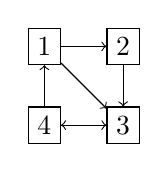
\begin{tikzpicture}
\tikzstyle{every node}+=[draw]
\tikzstyle{every edge}+=[->]

\node (1)              {1};
\node (2) [right of=1] {2};
\node (3) [below of=2] {3};
\node (4) [left of=3]  {4};

\path (1) edge             (2)
          edge             (3)
      (2) edge             (3)
      (3) edge             (4)
      (4) edge             (1)
          edge             (3);
\end{tikzpicture}
\end{exercise}
\end{frame}

\end{comment}

\subsection{Programmation \hadoop/}

\begin{frame}[fragile]{Java $\map$ for the term count example}
\begin{lstlisting}[language=java]
public class TermCountMapper extends MapReduceBase
  implements Mapper<Text,Text,Text,IntWritable> {
  public void map(
    Text uri, Text document,
    OutputCollector<Text, IntWritable> output,
    Reporter reporter)
  {
    Pattern p=Pattern.compile("[\\p{L}]+");
    Matcher m=p.matcher(document);
    while(matcher.find()) {
      String term=matcher.group().
      output.collect(new Text(term),new IntWritable(1));
    }
  }
}
\end{lstlisting}
\end{frame}

\begin{frame}[fragile]{Java $\reduce$ for the term count example}
\begin{lstlisting}[language=java]
public class TermCountReducer extends MapReduceBase
  implements Reducer<Text,IntWritable,Text,IntWritable> {
  public void reduce(
    Text term, Iterator<IntWritable> counts,
    OutputCollector<Text, IntWritable> output,
    Reporter reporter)
  {
    int sum=0;
    while(counts.hasNext()) {
      sum+=values.next().get();
    }
    output.collect(term, new IntWritable(sum));
  }
}
\end{lstlisting}
\end{frame}

\begin{frame}[fragile]{Java driver for the term count example}
\lstset{basicstyle=\footnotesize\ttfamily}
\begin{lstlisting}[language=java]
public class TermCount {
  public static void main(String args[]) throws IOException {
    JobConf conf = new JobConf(TermCount.class);
    FileInputFormat.addInputPath(conf, new Path(args[0]));
    FileOutputFormat.addOutputPath(conf, new Path(args[1]));

    // In a real application, we would have a custom input
    // format to fetch URI-document pairs
    conf.setInputFormat(KeyValueTextInputFormat.class);

    conf.setMapperClass(TermCountMapper.class);
    conf.setCombinerClass(TermCountReducer.class);
    conf.setReducerClass(TermCountReducer.class);

    conf.setOutputKeyClass(Text.class);
    conf.setOutputValueClass(IntWritable.class);

    JobClient.runJob(conf);
  }
}
\end{lstlisting}

\end{frame}

\section{Programmer facilement en \mapreduce/\,: \pig/}


\subsection{Basics}
\begin{frame}
\frametitle{Pig Latin}

\structure{Motivation:} définir un langage de haut niveau, type SQL,
qui s'appuie sur un moteur d'exécution \mapreduce/.

\vfill

Une ``requête'' \pig/ définit un opérateur qui prend une \alert{relation} en entrée
et produit une autre relation en sortie.

\vfill

Les requêtes consistent en une \alert{séquence} d'instructions 
suivant généralement le schéma suivant\,:

\begin{enumerate}
 \item  L'instruction \keyword{LOAD} charge les données d'un fichier (HDFS)
       sous la forme d'une \alert{relation} (liste de n-uplets).
   \item Une série de transformations traite les données.
   \item L'instruction (optionnelle) \keyword{STORE} écrit le résultat dans le système
       de fichiers (HDFS); on peut aussi faire un 
        \keyword{DUMP} pour afficher à l'écran.
\end{enumerate}

\vfill

Les requêtes sont evaluées par une \alert{combinaison} de \textit{jobs} \mapreduce/.
\end{frame}

\begin{frame}[fragile]
\frametitle{Tester \pig/}

\pig/ est un programme Java qui s'exécute en ligne de commande.
\begin{itemize}

\item Télécharger  depuis \url{http://pig.apache.org}.

\item Décompresser dans un répertoire, disons \texttt{pighome}

\item Placer le répertoire \texttt{pighome/bin} dans le chemin d'exécuton (\texttt{PATH})
\item Deux modes d'exécution
\begin{description}
\item[local] on lit les données sur le disque local, on évalue sans \mapreduce/ 
\item[MapReduce] on exécute dans un \textit{cluster} \mapreduce/, en lisant depuis HDFS.
\end{description}



\end{itemize}

Pour exécuter en local\,:
\begin{verbatim}
pig -x local
grunt>run <script>.pig
\end{verbatim}

\end{frame}

\begin{frame}[fragile]{Exemple de données en entrées (format tabulaire)}

Un fichier texte, un n-uplet par ligne, champs séparés par des tabulations.
\vfill
Fichier: \texttt{publishers.txt}
\footnotesize\begin{verbatim}
Fundations of Databases	Addison-Wesley	USA
Fundations of Databases	Vuibert	France
Web Data Management and Distribution	CUP	GB
\end{verbatim}

\vfill

Fichier: \texttt{books.txt}
\footnotesize\begin{verbatim}
1995	Fundations of Databases	Abiteboul
1995	Fundations of Databases	Hull
1995	Fundations of Databases	Vianu
2010	Web Data Management	Abiteboul
2010	Web Data Management	Manolescu
2010	Web Data Management	Rigaux
2010	Web Data Management	Rousset
2010	Web Data Management	Senellart
\end{verbatim}

\begin{block}{En pratique}
On peut écrire une fonction Java qui charge les données des fichiers et les transforme
en relation.
\end{block}
\end{frame}

\begin{frame}[fragile]
\frametitle{Premier exemple}

On regroupe les auteurs par livre.

\begin{lstlisting}[language=pig]
-- Chargement
books = load 'books.txt' 
    as (year: int, title: chararray, author: chararray) ;
    
-- Regroupement    
group_auth = group books by title;

-- Restruturation
authors = foreach group_auth generate group, books.author;

-- Affichage
dump authors;
\end{lstlisting}

\begin{block}{Exécution}
\begin{verbatim}
pig -x local
grunt>run groupby.pig
\end{verbatim}
\end{block}

\end{frame}

\begin{frame}[fragile]
\frametitle{Modèle de données}

Modèle semi-structuré, type XML/JSON. Imbrication de structures ensemblistes (``bags'') et de n-uplets.

\vfill

Exemple: le bag \texttt{group\_auth}.

{\small\begin{verbatim}
(
  Fundations of Databases,
  { (1995,Fundations of Databases,Abiteboul),
    (1995,Fundations of Databases,Hull),
    (1995,Fundations of Databases,Vianu)
  }
)
\end{verbatim}
}

Imbrication sans limite, mais pas de références ou dépendance externe\,: un ``document'' autonome. 
\alert{Objectif parallélisation}\,!

\vfill

Les champs peuvent être référencés par leur nom (quand il y a un schéma) ou par leur position (ex, \texttt{\$1}).
\end{frame}

\subsection{Les opérateurs \pig/}

\begin{frame}[fragile]
\frametitle{Principaux opérateurs \pig/}

\begin{small}
\begin{tabular}{lp{9cm}}
\toprule
\textbf{Operator} & \textbf{Description} \\
\midrule
\keyword{foreach} &  Apply one or several expression(s) to each of the input
tuples\\ 
\keyword{filter} &  Filtre les tuples sur certains critères\\ 
\keyword{distinct} &  Elimination des doublons\\ 
\keyword{join} &  Jointures de deux \textit{bags}\\ 
\keyword{group} & Regroupement \\
\keyword{cogroup} & Association de n-uplets provenant de deux sources\\ 
\keyword{cross} &  Produit cartésien de deux sources\\ 
\keyword{order} & Tri\\ 
\keyword{limit} & Limite la taille des données traitées\\
\keyword{union} &  Union de deux sources (dont les schémas peuvent être très différents)\\ 
\keyword{split} & Partition d'une relation selon certains critères\\
\bottomrule
\end{tabular}
\end{small}

\end{frame}




\begin{frame}[fragile]
\frametitle{Opérateur de ``dégroupage''}

\texttt{flatten} ``déploie'' une imbrication (\texttt{flatten.pig}).

\begin{lstlisting}[language=pig]
-- Take the `authors' bag and flatten the nested set
flattened = foreach authors  
  generate group, flatten($1);
\end{lstlisting}

\vfill

Appliqué à la relation  \texttt{authors} créée précédemment, on obtient\,:


\small\begin{verbatim}
(Foundations of Databases,Abiteboul)
(Foundations of Databases,Hull)
(Foundations of Databases,Vianu)
(Web Data Management,Abiteboul)
(Web Data Management,Manolescu)
(Web Data Management,Rigaux)
(Web Data Management,Rousset)
(Web Data Management,Senellart)
\end{verbatim}
\end{frame}


\begin{frame}[fragile]
\frametitle{L'opérateur \texttt{cogroup}}

\vfill
Permet d'assembler des n-uplets sur un ensemble de critères.

\vfill
Exemple (\texttt{cogroup.pig})\,:

\begin{lstlisting}[language=pig]
publishers = load 'publishers.txt' 
    as (title: chararray, publisher: chararray) ;
cogrouped = cogroup flattened by group,
                    publishers by title;
\end{lstlisting}

\end{frame}


\begin{frame}[fragile]
\frametitle{Résultat (mis en forme)}
\vfill
Pour chaque valeur de regroupement, deux ensembles imbriqués,
provenant de chacune des sources.

\vfill

{\small\begin{verbatim}
(Foundations of Databases,
  { (Foundations of Databases,Abiteboul),
    (Foundations of Databases,Hull),
    (Foundations of Databases,Vianu)
  },
  {(Foundations of Databases,Addison-Wesley),
   (Foundations of Databases,Vuibert)
  }
)
\end{verbatim}
}

\vfill
Une sorte de jointure, dans un état intermédiaire, permis par le modèle semim-structuré.

\end{frame}


\begin{frame}[fragile]
\frametitle{Jointures}
\vfill
Come précédemment, mais produit un résultat ``mis à plat''. 

\vfill

On
effectue le produit cartésien des n-uplets imbriqués (\texttt{join.pig}).

\vfill

\begin{lstlisting}[language=pig]
-- Take the 'flattened' bag, join with 'publishers'
joined = join flattened by group, publishers by title;
\end{lstlisting}

\vfill

{\small\begin{verbatim}
(Foundations of Databases,Abiteboul,
      Fundations of Databases,Addison-Wesley)
(Foundations of Databases,Abiteboul,
      Fundations of Databases,Vuibert)
(Foundations of Databases,Hull,
      Fundations of Databases,Addison-Wesley)
(Foundations of Databases,Hull,
     ...
\end{verbatim}
}

\end{frame}


\begin{frame}[fragile]
\frametitle{Un exemple complet}
\vfill
Avec ajout de filtres pour sélectionner certain n-uplets.


\vfill

\begin{lstlisting}[language=pig]
-- Chargement de books.txt
books = load 'books.txt' 
    as (year: int, title: chararray, author: chararray) ;
-- On prend les livres de Victor Vianu
vianu = filter books by author == 'Vianu';
--- Chargement de publishers.txt
publishers = load 'publishers.txt' 
    as (title: chararray, publisher: chararray) ;
-- Jointure sur le titre
joined = join vianu by title, publishers by title;
-- Groupement sur le nom de l'auteur
grouped = group joined by vianu::author;
-- Maintenant, comptons les editeurs (exercice: supprimer les doublons!)
count = foreach grouped generate group, COUNT(joined.publisher);
\end{lstlisting}

À tester (\texttt{join-and-group.pig})...

\end{frame}


\subsection{De Pig à MapReduce}


\begin{frame}{Les opérateurs physiques}

\begin{description}
\item[Local Rearrange] regroupement des n-uplets avec la même clé, sur la machine locale. 

\item[Global Rearrange] regroupement des tuples avec la même clé, dans le système distribué

\item[Package] construction d'un n-uplet  à partir de n-uplets regroupés.
\end{description}

\end{frame}

\begin{frame}{Traduction d'un programme Pig en MapReduce}

Premier exemple\,: regroupement des livres sur le titre.

\figSlideWithSize{pigeval-1}{\linewidth}

Correspond à un programme MapReduce assez direct.

\end{frame}


\begin{frame}{Traduction du programme \texttt{join-group}}

La jointure implique un premier MapReduce

\vfill

\figSlideWithSize{pigeval-2}{\linewidth}

\vfill

Le group-by implique un second MapReduce.

\begin{block}{Bilan}
Ca va prendre du temps...
\end{block}
\end{frame}

\section{Quelques conclusions}

\begin{frame}{MapReduce: puissant et limité à la fois (1/2)}

\begin{itemize}

\item \alert{Très forte latence.} Démarre une programe \mapreduce/ prend
\alert{beaucoup} de temps\,; la fonction $\reduce$ n'est appliquée
que quand tous les $\map$ ont terminé.

    $\Rightarrow$ ça prend des heures ou de jours.
    

\item \alert{Traitement par lor seulement.} \mapreduce/ est bon
   pour traiter de très grandes collections, par pour identifier
     rapidement certains éléments.

\item \alert{J'écris une fois, je lis plusieurs fois.} Pas de mise à jour
  avec \mapreduce/.

\item \alert{Pas de transaction.} 

\end{itemize}
\end{frame}

\begin{frame}{Limitations de MapReduce, suite   (2/2)}
\begin{itemize}
\item \alert{C'est de la programmation.} Parmi les langages de plus haut niveau: Scope, Pig,
 Hive, Cascading, ...

\item \alert{Aucune structure, aucun contrôle}. Hum...

\item \alert{Difficile à régler.} Combien de \textit{reducers}, combien de mémoire
sur chaque n{\oe}uds, où utiliser la compression, etc.

\end{itemize}

\end{frame}
